\part{Segundo semestre}
\chapterimage{2.pdf}
\chapter{Álgebra II}


\section{Función lineal} %(1.5 semanas)
En esta unidad se abordarán los conceptos fundamentales relacionados con las funciones lineales, incluyendo su definición general, la relación con la variación directamente proporcional, y las técnicas para tabular y graficar estas funciones.

\subsection{Concepto general de función}

Una función es una relación matemática entre dos conjuntos de números, donde a cada elemento del primer conjunto (dominio) le corresponde exactamente un elemento del segundo conjunto (codominio). Formalmente, una función \( f \) se define como un conjunto de pares ordenados \((x, f(x))\), donde \(x\) es el valor de entrada y \(f(x)\) es el valor de salida. La función lineal es un caso específico de función que se puede expresar en la forma general:
\begin{equation}
    f(x) = mx + b
\end{equation}

donde \(m\) es la pendiente de la recta y \(b\) es la ordenada al origen.

\subsection{Variación directamente proporcional}

La variación directamente proporcional es un tipo especial de relación entre dos variables \(x\) e \(y\), donde \(y\) varía en la misma proporción que \(x\). Matemáticamente, esto se expresa como:

\[
y = kx
\]

donde \(k\) es la constante de proporcionalidad. Esta relación representa una función lineal con pendiente \(k\) y ordenada al origen \(b = 0\).

\subsection{Función Lineal}

Una función lineal es aquella que se puede representar en la forma general:

\[
f(x) = mx + b
\]

donde:
\begin{itemize}
    \item \(m\) es la pendiente de la recta, que indica la tasa de cambio de la función.
    \item \(b\) es la ordenada al origen, el valor de \(f(x)\) cuando \(x = 0\).
\end{itemize}

La pendiente \(m\) se calcula como la relación entre el cambio en \(y\) y el cambio en \(x\):
\begin{equation}
    m = \frac{\Delta y}{\Delta x}
\end{equation}

La función lineal produce una gráfica en forma de recta. La pendiente determina la inclinación de la recta y la ordenada al origen determina el punto donde la recta cruza el eje \(y\).

\subsection{Tabular y graficar funciones lineales}

Para tabular y graficar una función lineal, se siguen estos pasos:

\begin{enumerate}
    \item \textbf{Determinar la función lineal} \(f(x) = mx + b\).
    
    \item \textbf{Elegir valores de \(x\)} para los cuales se calcularán los valores correspondientes de \(f(x)\). Por ejemplo, si \(f(x) = 2x + 3\), elige valores como \(x = -1, 0, 1, 2\).
    
    \item \textbf{Calcular los valores} de \(f(x)\) para los valores elegidos de \(x\). Para \(x = -1\), \(f(-1) = 2(-1) + 3 = 1\).
    
    \item \textbf{Construir una tabla} con los pares ordenados \((x, f(x))\):

    \[
    \begin{array}{|c|c|}
    \hline
    x & f(x) \\
    \hline
    -1 & 1 \\
    0 & 3 \\
    1 & 5 \\
    2 & 7 \\
    \hline
    \end{array}
    \]

    \item \textbf{Graficar los puntos} en un plano cartesiano y dibujar la recta que pasa por todos ellos.
    
    \item \textbf{Interpretar la gráfica} para obtener información sobre la pendiente y la ordenada al origen de la función lineal.
\end{enumerate}

\begin{center}
    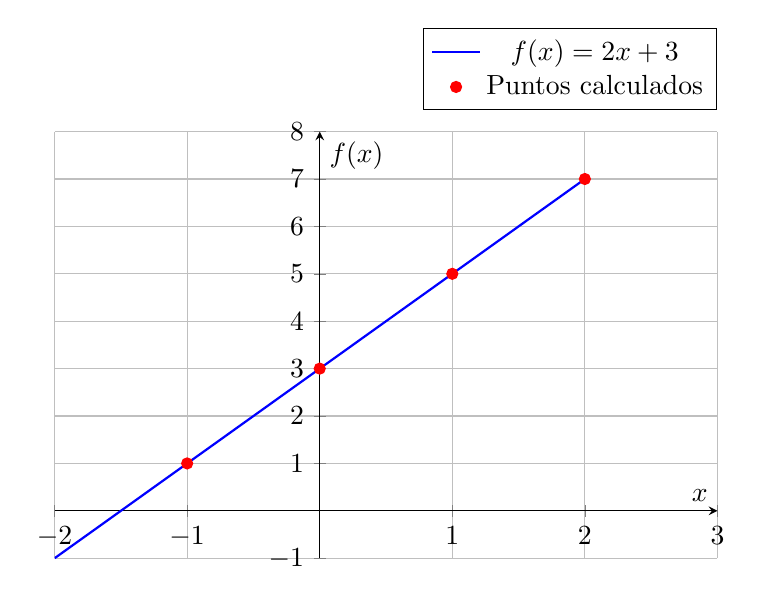
\begin{tikzpicture}
        \begin{axis}[
            axis lines = middle,
            xlabel = {$x$},
            ylabel = {$f(x)$},
            xmin = -2, xmax = 3,
            ymin = -1, ymax = 8,
            xtick = {-2,-1,0,1,2,3},
            ytick = {-1,0,1,2,3,4,5,6,7,8},
            grid = both,
            legend style={at={(1,1.05)}, anchor=south east},
            width=10cm, height=7cm
        ]
        % Gráfica de la función lineal
        \addplot[
            domain=-2:2, 
            samples=100,
            thick,
            blue
        ]
        {2*x + 3};
        \addlegendentry{$f(x) = 2x + 3$}
        
        % Puntos específicos
        \addplot[only marks, mark=*, red] coordinates {(-1,1) (0,3) (1,5) (2,7)};
        \addlegendentry{Puntos calculados}
        \end{axis}
    \end{tikzpicture}
    \end{center}






    \section{Sistema de Ecuaciones Lineales} %(4 semanas)

    En esta unidad, se explorarán los conceptos fundamentales y métodos para resolver sistemas de ecuaciones lineales, así como sus aplicaciones prácticas.
    
    \subsection{Conceptos Básicos}
    
    \subsubsection{Concepto de Sistema de Ecuaciones}
    
    Un sistema de ecuaciones lineales es un conjunto de dos o más ecuaciones que comparten las mismas variables. La solución del sistema es el conjunto de valores de las variables que satisface todas las ecuaciones simultáneamente.
    
    \subsubsection{Concepto de Solución de un Sistema de Ecuaciones Lineales}
    
    La solución de un sistema de ecuaciones lineales es el conjunto de valores de las variables que hace que todas las ecuaciones del sistema sean verdaderas al mismo tiempo.
    
    \subsubsection{Concepto de Solución Consistente, Inconsistente y Dependiente}
    
    Consistente: Un sistema es consistente si tiene al menos una solución.
    Inconsistente: Un sistema es inconsistente si no tiene soluciones.
    Dependiente: Un sistema es dependiente si tiene infinitas soluciones.
    \subsection{Operaciones y Procedimientos}
    
    \subsubsection{Métodos de Solución de Sistemas}
    
    Existen varios métodos para resolver sistemas de ecuaciones lineales:
    
    \begin{itemize}
    \item Igualación
    \item Sustitución
    \item Reducción (Eliminación, Sumas o Restas)
    \item Determinantes
    \item Gráfica
    \end{itemize}
    
    \subsubsection{Igualación}
    
    El método de igualación consiste en despejar una de las variables en ambas ecuaciones y luego igualar las expresiones obtenidas.
    
    \textbf{Procedimiento:}
    \begin{enumerate}
        \item \textbf{Despejar una variable:} Despeja la misma variable en ambas ecuaciones.
        \item \textbf{Igualar las expresiones:} Igualar las dos expresiones obtenidas para esa variable.
        \item \textbf{Resolver:} Resuelve la ecuación resultante para obtener el valor de la variable.
        \item \textbf{Sustituir:} Sustituye el valor encontrado en una de las ecuaciones originales para obtener el valor de la otra variable.
    \end{enumerate}
    
    \textbf{Ejemplo:}
    
    Considera el siguiente sistema de ecuaciones:
    \[
    \begin{cases}
    2x + y = 7 \\
    3x - y = 4
    \end{cases}
    \]
    
    \begin{enumerate}
        \item \textbf{Despejar la variable \(y\) en ambas ecuaciones:}
            \[
            y = 7 - 2x
            \]
            \[
            y = 3x - 4
            \]
        \item \textbf{Igualar las dos expresiones para \(y\):}
            \[
            7 - 2x = 3x - 4
            \]
        \item \textbf{Resolver para \(x\):}
            \[
            7 + 4 = 3x + 2x \implies 11 = 5x \implies x = \frac{11}{5}
            \]
        \item \textbf{Sustituir \(x = \frac{11}{5}\) en una de las ecuaciones originales:}
            \[
            y = 7 - 2 \left(\frac{11}{5}\right) = 7 - \frac{22}{5} = \frac{35 - 22}{5} = \frac{13}{5}
            \]
    \end{enumerate}
    
    \textbf{Solución:} \( \left( \frac{11}{5}, \frac{13}{5} \right) \)
    
     
    
    \subsubsection{Sustitución}
    
    El método de sustitución implica resolver una de las ecuaciones para una de las variables y luego sustituir esta expresión en la otra ecuación.
    
    \textbf{Procedimiento:}
    \begin{enumerate}
        \item \textbf{Despejar una variable:} Despeja una de las variables en una de las ecuaciones.
        \item \textbf{Sustituir:} Sustituye la expresión obtenida en la otra ecuación.
        \item \textbf{Resolver:} Resuelve la ecuación resultante para obtener el valor de una variable.
        \item \textbf{Sustituir el valor encontrado:} Sustituye el valor de la variable obtenida en la ecuación inicial para encontrar el valor de la otra variable.
    \end{enumerate}
    
    \textbf{Ejemplo:}
    
    Considera el siguiente sistema de ecuaciones:
    \[
    \begin{cases}
    x + y = 8 \\
    2x - y = 3
    \end{cases}
    \]
    
    \begin{enumerate}
        \item \textbf{Despejar la variable \(y\) en la primera ecuación:}
            \[
            y = 8 - x
            \]
        \item \textbf{Sustituir en la segunda ecuación:}
            \[
            2x - (8 - x) = 3
            \]
            \[
            2x - 8 + x = 3 \implies 3x - 8 = 3 \implies 3x = 11 \implies x = \frac{11}{3}
            \]
        \item \textbf{Sustituir \(x = \frac{11}{3}\) en la ecuación \(y = 8 - x\):}
            \[
            y = 8 - \frac{11}{3} = \frac{24 - 11}{3} = \frac{13}{3}
            \]
    \end{enumerate}
    
    \textbf{Solución:} \( \left( \frac{11}{3}, \frac{13}{3} \right) \)
    
     
    
    \subsubsection{Reducción (Eliminación, Sumas o Restas)}
    
    El método de reducción o eliminación se basa en sumar o restar las ecuaciones para eliminar una de las variables.
    
    
    \textbf{Procedimiento:}
    \begin{enumerate}
        \item \textbf{Multiplicar las ecuaciones:} Si es necesario, multiplica las ecuaciones para que los coeficientes de una de las variables sean opuestos.
        \item \textbf{Sumar o restar las ecuaciones:} Suma o resta las ecuaciones para eliminar una variable.
        \item \textbf{Resolver la ecuación resultante:} Resuelve para la variable restante.
        \item \textbf{Sustituir:} Sustituye el valor obtenido en una de las ecuaciones originales para encontrar el valor de la otra variable.
    \end{enumerate}
    
    \textbf{Ejemplo:}
    
    Considera el siguiente sistema de ecuaciones:
    \[
    \begin{cases}
    4x + 3y = 10 \\
    2x - 3y = 1
    \end{cases}
    \]
    
    \begin{enumerate}
        \item \textbf{Sumar las ecuaciones (ya están listas para ser sumadas):}
            \[
            (4x + 3y) + (2x - 3y) = 10 + 1
            \]
            \[
            6x = 11 \implies x = \frac{11}{6}
            \]
        \item \textbf{Sustituir \(x = \frac{11}{6}\) en una de las ecuaciones originales:}
            \[
            4 \left(\frac{11}{6}\right) + 3y = 10
            \]
            \[
            \frac{44}{6} + 3y = 10 \implies 3y = 10 - \frac{44}{6}
            \]
            \[
            3y = \frac{60 - 44}{6} = \frac{16}{6} \implies y = \frac{16}{18} = \frac{8}{9}
            \]
    \end{enumerate}
    
    \textbf{Solución:} \( \left( \frac{11}{6}, \frac{8}{9} \right) \)
    
     
    \subsubsection{Determinantes}
    
    Para sistemas de ecuaciones lineales de $n$ ecuaciones con $n$ incógnitas, se pueden utilizar determinantes para encontrar soluciones.
    
    \textbf{Procedimiento:}
    \begin{enumerate}
        \item \textbf{Formar la matriz:} Escribe el sistema de ecuaciones en forma de matriz aumentada.
        \item \textbf{Calcular el determinante:} Usa la regla de Cramer o matrices inversas para calcular el determinante y encontrar las soluciones.
    \end{enumerate}
    
    \textbf{Ejemplo:}
    
    Considera el siguiente sistema de ecuaciones:
    \[
    \begin{cases}
    x + y = 4 \\
    2x - y = 1
    \end{cases}
    \]
    
    \begin{enumerate}
        \item \textbf{Formar la matriz:}
            \[
            A = \begin{pmatrix}
            1 & 1 \\
            2 & -1
            \end{pmatrix}, \quad \textbf{b} = \begin{pmatrix}
            4 \\
            1
            \end{pmatrix}
            \]
        \item \textbf{Calcular el determinante de \(A\):}
            \[
            \text{Det}(A) = (1 \cdot (-1)) - (1 \cdot 2) = -1 - 2 = -3
            \]
    
            \textbf{Determinantes para \(x\) y \(y\):}
            \[
            A_x = \begin{pmatrix}
            4 & 1 \\
            1 & -1
            \end{pmatrix} \implies \text{Det}(A_x) = (4 \cdot (-1)) - (1 \cdot 1) = -4 - 1 = -5
            \]
            \[
            A_y = \begin{pmatrix}
            1 & 4 \\
            2 & 1
            \end{pmatrix} \implies \text{Det}(A_y) = (1 \cdot 1) - (4 \cdot 2) = 1 - 8 = -7
            \]
    
        \item \textbf{Calcular las soluciones:}
            \[
            x = \frac{\text{Det}(A_x)}{\text{Det}(A)} = \frac{-5}{-3} = \frac{5}{3}
            \]
            \[
            y = \frac{\text{Det}(A_y)}{\text{Det}(A)} = \frac{-7}{-3} = \frac{7}{3}
            \]
    \end{enumerate}
    
    \textbf{Solución:} \( \left( \frac{5}{3}, \frac{7}{3} \right) \)
    
     
    
    \subsubsection{Gráfica de Sistema de Ecuaciones Lineales de Dos Variables}
    
    Para sistemas de dos ecuaciones lineales con dos variables, las ecuaciones se pueden representar gráficamente como líneas en un plano cartesiano. La intersección de estas líneas representa la solución del sistema.
    
    \begin{center}
    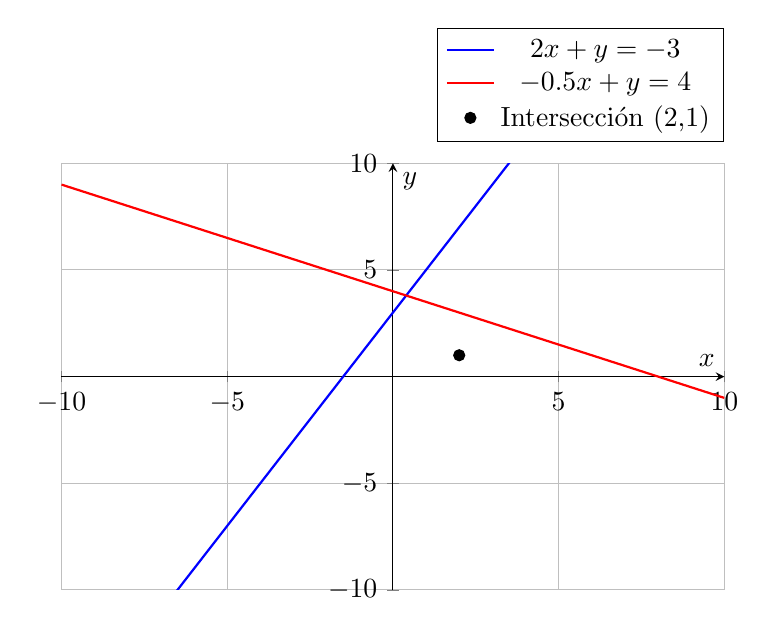
\begin{tikzpicture}
    \begin{axis}[
    axis lines = middle,
    xlabel = {$x$},
    ylabel = {$y$},
    xmin = -10, xmax = 10,
    ymin = -10, ymax = 10,
    xtick = {-10,-5,0,5,10},
    ytick = {-10,-5,0,5,10},
    grid = both,
    legend style={at={(1,1.05)}, anchor=south east},
    width=10cm, height=7cm
    ]
    % Ecuación 1
    \addplot[
    domain=-10:10,
    samples=100,
    thick,
    blue
    ]
    {2*x + 3};
    \addlegendentry{$2x + y = -3$}
    % Ecuación 2
    \addplot[ domain=-10:10,    samples=100,    thick,    red]
    {-0.5*x + 4};
    \addlegendentry{$-0.5x + y = 4$}
    
    % Punto de intersección
    \addplot[only marks, mark=*, black] coordinates {(2, 1)};
    \addlegendentry{Intersección (2,1)}
    \end{axis}
    \end{tikzpicture}
    \end{center}
    
    \textbf{Procedimiento:}
    \begin{enumerate}
        \item \textbf{Graficar cada ecuación:} Encuentra dos puntos para cada línea y dibuja las líneas correspondientes.
        \item \textbf{Encontrar la intersección:} La solución al sistema es el punto donde las líneas se cruzan.
    \end{enumerate}
    
    \textbf{Ejemplo:}
    
    Considera el siguiente sistema de ecuaciones:
    \[
    \begin{cases}
    x + y = 4 \\
    x - y = 2
    \end{cases}
    \]
    
    \begin{enumerate}
        \item \textbf{Graficar las ecuaciones:}
            \begin{itemize}
                \item Para \(x + y = 4\):
                    \[
                    \text{Cuando } x = 0, \, y = 4
                    \]
                    \[
                    \text{Cuando } x = 4, \, y = 0
                    \]
                    \[
                    \text{Dibuja la línea que pasa por (0,4) y (4,0)}
                    \]
    
                \item Para \(x - y = 2\):
                    \[
                    \text{Cuando } x = 0, \, y = -2
                    \]
                    \[
                    \text{Cuando } x = 2, \, y = 0
                    \]
                    \[
                    \text{Dibuja la línea que pasa por (0,-2) y (2,0)}
                    \]
            \end{itemize}
    
        \item \textbf{Encontrar la intersección:}
    
            Al graficar las líneas, observamos que se cruzan en el punto \((3, 1)\).
    \end{enumerate}
    
    \textbf{Solución:} \( (3, 1) \)
    \begin{tikzpicture}[scale=1.2]
        % Ejes
        \draw[->] (-1,0) -- (5,0) node[right] {$x$};
        \draw[->] (0,-1) -- (0,5) node[above] {$y$};
        
        % Ecuación x + y = 4
        \draw[blue, thick] (-1,5) -- (5,-1) node[right] {$x + y = 4$};
        
        % Ecuación x - y = 2
        \draw[red, thick] (0, -2) -- (4, 2) node[right] {$x - y = 2$};
        
        % Punto de intersección
        \fill[black] (3,1) circle (2pt);
        \node at (3, 1.3) {$(3, 1)$};
        
        % Etiquetas
        \node at (4.5, 4.5) {$(x + y = 4)$};
        \node at (4, -1) {$(x - y = 2)$};
        
        % Rejilla
        \foreach \x in {1,2,3,4} \draw (\x,1pt) -- (\x,-1pt) node[below] {\x};
        \foreach \y in {1,2,3,4} \draw (1pt,\y) -- (-1pt,\y) node[left] {\y};
    \end{tikzpicture}
    
    \subsection{Aplicaciones y Problemas}
    
    \subsubsection{Plantear y Resolver Problemas}
    
    Los sistemas de ecuaciones lineales se aplican en diversos contextos, como en la resolución de problemas de mezcla, planificación de recursos y modelado de datos.
    
    \subsubsection{Empleo de un Sistema de Ecuaciones Lineales}
    
    En aplicaciones prácticas, los sistemas de ecuaciones lineales pueden modelar situaciones donde se necesita encontrar soluciones que satisfagan múltiples restricciones simultáneamente.
    
    
    
     
    
    \subsubsection{Ejemplo: Mezcla de Productos}
    
    \textbf{Problema:} Un fabricante de mezclas tiene dos tipos de productos: A y B. El producto A cuesta \$5 por litro y el producto B cuesta \$8 por litro. El fabricante desea preparar 100 litros de una mezcla que debe costar \$6 por litro. ¿Cuántos litros de cada tipo de producto debe usar?
    
    \textbf{Solución:}
    
    Sea \( x \) la cantidad de litros del producto A y \( y \) la cantidad de litros del producto B. Entonces, tenemos dos ecuaciones:
    
    \begin{itemize}
        \item La ecuación para el total de litros es:
        \[
        x + y = 100
        \]
        \item La ecuación para el costo total de la mezcla es:
        \[
        5x + 8y = 6 \times 100
        \]
    \end{itemize}
    
    Resolviendo el sistema de ecuaciones:
    
    \[
    \begin{cases}
    x + y = 100 \\
    5x + 8y = 600
    \end{cases}
    \]
    
    Multiplicamos la primera ecuación por 5:
    
    \[
    5x + 5y = 500
    \]
    
    Restamos esta ecuación de la segunda ecuación:
    
    \[
    (5x + 8y) - (5x + 5y) = 600 - 500 \\
    3y = 100 \\
    y = \frac{100}{3} \approx 33.33
    \]
    
    Sustituyendo \( y = 33.33 \) en la primera ecuación:
    
    \[
    x + 33.33 = 100 \\
    x = 100 - 33.33 = 66.67
    \]
    
    Por lo tanto, se deben usar aproximadamente 66.67 litros del producto A y 33.33 litros del producto B.
    
    \subsection{Planificación de Recursos: Asignación de Tareas}
    
    \textbf{Problema:} Una empresa debe asignar tres tareas a dos trabajadores. La tarea 1 toma 4 horas, la tarea 2 toma 3 horas y la tarea 3 toma 2 horas. Los trabajadores tienen disponibles 8 horas cada uno. ¿Cómo deben asignarse las tareas para que se utilicen al máximo las horas disponibles?
    
    \textbf{Solución:}
    
    Sea \( x_1 \), \( x_2 \), y \( x_3 \) la cantidad de horas dedicadas a las tareas 1, 2 y 3 por el Trabajador 1, y \( y_1 \), \( y_2 \), y \( y_3 \) la cantidad de horas dedicadas a las mismas tareas por el Trabajador 2. Entonces:
    
    \begin{itemize}
        \item La ecuación para las horas disponibles de cada trabajador es:
        \[
        4x_1 + 3x_2 + 2x_3 \leq 8
        \]
        \[
        4y_1 + 3y_2 + 2y_3 \leq 8
        \]
        \item La ecuación para completar todas las tareas es:
        \[
        x_1 + y_1 = 1 \\
        x_2 + y_2 = 1 \\
        x_3 + y_3 = 1
        \]
    \end{itemize}
    
    Podemos resolver este problema mediante programación lineal. Si el objetivo es maximizar el uso de horas disponibles, se plantea como un problema de maximización sujeto a las restricciones anteriores.
    
    
    \subsection{Modelado de Datos: Ajuste de Modelo Lineal}
    
    \textbf{Problema:} Un analista desea modelar la relación entre el tiempo (en horas) dedicado al estudio y la calificación obtenida en un examen. Se recopilan los siguientes datos:
    
    \[
    \begin{array}{|c|c|}
    \hline
    \text{Horas de Estudio} & \text{Calificación} \\
    \hline
    1 & 60 \\
    2 & 65 \\
    3 & 70 \\
    4 & 75 \\
    5 & 80 \\
    \hline
    \end{array}
    \]
    
    Se desea ajustar un modelo lineal \( y = mx + b \) a estos datos.
    
    \textbf{Solución:}
    
    Se utiliza el método de mínimos cuadrados para encontrar los valores de \( m \) y \( b \). Primero calculamos las medias de \( x \) y \( y \), y luego las sumas requeridas:
    
    \[
    \bar{x} = \frac{1+2+3+4+5}{5} = 3
    \]
    \[
    \bar{y} = \frac{60+65+70+75+80}{5} = 70
    \]
    
    Las fórmulas para \( m \) y \( b \) son:
    
    \[
    m = \frac{\sum (x_i - \bar{x})(y_i - \bar{y})}{\sum (x_i - \bar{x})^2}
    \]
    \[
    b = \bar{y} - m \bar{x}
    \]
    
    Calculamos:
    \begin{align*}
    &\sum (x_i - \bar{x})(y_i - \bar{y}) =\\
    &(1-3)(60-70) + (2-3)(65-70) + (3-3)(70-70) + (4-3)(75-70) + (5-3)(80-70) =\\
    &40 + 5 + 0 + 5 + 20 = 70
    \end{align*}
    
    \[
    \sum (x_i - \bar{x})^2 = (1-3)^2 + (2-3)^2 + (3-3)^2 + (4-3)^2 + (5-3)^2 = 4 + 1 + 0 + 1 + 4 = 10
    \]
    
    \[
    m = \frac{70}{10} = 7
    \]
    
    \[
    b = 70 - 7 \times 3 = 49
    \]
    
    El modelo ajustado es \( y = 7x + 49 \).





    \section{Ecuaciones Cuadráticas} % (3 semanas)

    \subsection{Ecuaciones Cuadráticas y Sus Raíces o Soluciones}
    
    Una ecuación cuadrática tiene la forma general:
    \begin{equation}
        ax^2 + bx + c = 0
    \end{equation}
    donde \(a\), \(b\), y \(c\) son constantes y \(a \neq 0\). Las soluciones de una ecuación cuadrática se obtienen resolviendo para \(x\).
    
    \subsection{La Propiedad del Producto Cero y la Resolución de Ecuaciones por Factorización}
    
    \textbf{Propiedad del Producto Cero:} Si el producto de dos factores es cero, al menos uno de los factores debe ser cero. Esto se expresa como:
    \[
    ab = 0 \implies a = 0 \text{ o } b = 0
    \]
    
    \textbf{Ejemplo de Factorización:} Considera la ecuación cuadrática:
    \[
    x^2 - 5x + 6 = 0
    \]
    Para resolverla por factorización, buscamos dos números que multiplicados den 6 y sumados den -5. Estos números son -2 y -3, por lo que:
    \[
    x^2 - 5x + 6 = (x - 2)(x - 3) = 0
    \]
    Aplicando la propiedad del producto cero:
    \[
    x - 2 = 0 \text{ o } x - 3 = 0
    \]
    \[
    x = 2 \text{ o } x = 3
    \]
    
    \subsection{Solución de Ecuaciones Cuadráticas Completando el Trinomio Cuadrado Perfecto}
    
    Para resolver una ecuación cuadrática completando el trinomio cuadrado perfecto, transformamos la ecuación en la forma:
    \[
    x^2 + bx = -c
    \]
    Añadimos y restamos \(\left(\frac{b}{2}\right)^2\) para completar el cuadrado:
    \[
    x^2 + bx + \left(\frac{b}{2}\right)^2 = \left(\frac{b}{2}\right)^2 - c
    \]
    \[
    \left(x + \frac{b}{2}\right)^2 = \left(\frac{b}{2}\right)^2 - c
    \]
    Luego resolvemos:
    \[
    x + \frac{b}{2} = \pm \sqrt{\left(\frac{b}{2}\right)^2 - c}
    \]
    \[
    x = -\frac{b}{2} \pm \sqrt{\left(\frac{b}{2}\right)^2 - c}
    \]
    
    \textbf{Ejemplo:} Para \(x^2 - 4x - 5 = 0\):
    \[
    x^2 - 4x = 5
    \]
    Añadimos \(\left(\frac{-4}{2}\right)^2 = 4\):
    \[
    x^2 - 4x + 4 = 5 + 4
    \]
    \[
    (x - 2)^2 = 9
    \]
    \[
    x - 2 = \pm 3
    \]
    \[
    x = 2 \pm 3
    \]
    \[
    x = 5 \text{ o } x = -1
    \]
    
    \subsection{Resolución de Ecuaciones Cuadráticas por la Fórmula General}
    
    La fórmula general para resolver una ecuación cuadrática \(ax^2 + bx + c = 0\) es:
    \[
    x = \frac{-b \pm \sqrt{b^2 - 4ac}}{2a}
    \]
    
    \textbf{Ejemplo:} Para la ecuación \(2x^2 - 4x - 6 = 0\):
    \[
    a = 2, \quad b = -4, \quad c = -6
    \]
    \[
    x = \frac{-(-4) \pm \sqrt{(-4)^2 - 4 \cdot 2 \cdot (-6)}}{2 \cdot 2}
    \]
    \[
    x = \frac{4 \pm \sqrt{16 + 48}}{4}
    \]
    \[
    x = \frac{4 \pm \sqrt{64}}{4}
    \]
    \[
    x = \frac{4 \pm 8}{4}
    \]
    \[
    x = 3 \text{ o } x = -1
    \]
    
    \subsection{El Discriminante de una Ecuación Cuadrática y el Tipo de Raíces}
    
    El discriminante de una ecuación cuadrática \(ax^2 + bx + c = 0\) es:
    \[
    \Delta = b^2 - 4ac
    \]
    El discriminante nos indica el tipo de raíces:
    \begin{itemize}
        \item \(\Delta > 0\): Dos raíces reales y distintas.
        \item \(\Delta = 0\): Una raíz real doble.
        \item \(\Delta < 0\): Dos raíces complejas conjugadas.
    \end{itemize}
    
    \textbf{Ejemplo:} Para la ecuación \(x^2 - 4x + 4 = 0\):
    \[
    a = 1, \quad b = -4, \quad c = 4
    \]
    \[
    \Delta = (-4)^2 - 4 \cdot 1 \cdot 4 = 16 - 16 = 0
    \]
    \textbf{Tipo de Raíces:} Una raíz real doble, \(x = 2\).
    
    \subsection{Solución de Ecuaciones Reducibles a Cuadráticas Mediante un Cambio de Variable}
    
    Algunas ecuaciones pueden ser reducidas a una cuadrática mediante un cambio de variable. Por ejemplo, para la ecuación:
    \[
    x^4 - 5x^2 + 4 = 0
    \]
    Hacemos el cambio de variable \(y = x^2\), así que la ecuación se convierte en:
    \[
    y^2 - 5y + 4 = 0
    \]
    Resolviendo esta cuadrática:
    \[
    (y - 4)(y - 1) = 0
    \]
    \[
    y = 4 \text{ o } y = 1
    \]
    Deshacemos el cambio de variable:
    \[
    x^2 = 4 \implies x = \pm 2
    \]
    \[
    x^2 = 1 \implies x = \pm 1
    \]
    
    \subsection{Resolución de Ecuaciones que Contienen Radicales}
    
    Para resolver ecuaciones que contienen radicales, es útil aislar el radical y luego elevar ambos lados de la ecuación al cuadrado para eliminar el radical.
    
    \textbf{Ejemplo:} Resolvamos la ecuación:
    \[
    \sqrt{x + 3} = x - 1
    \]
    Elevamos ambos lados al cuadrado:
    \[
    x + 3 = (x - 1)^2
    \]
    \[
    x + 3 = x^2 - 2x + 1
    \]
    \[
    0 = x^2 - 3x - 2
    \]
    Resolviendo esta cuadrática por factorización:
    \[
    (x - 2)(x - 1) = 0
    \]
    \[
    x = 2 \text{ o } x = 1
    \]
    Verificamos las soluciones en la ecuación original:
    \[
    \text{Para } x = 2: \sqrt{2 + 3} = 2 - 1 \quad \text{es cierto.}
    \]
    \[
    \text{Para } x = 1: \sqrt{1 + 3} = 1 - 1 \quad \text{no es cierto.}
    \]
    \textbf{Solución final:} \(x = 2\).






    \section{Funciones y Desigualdades Cuadráticas} % (4 semanas)

    \subsection{Funciones Cuadráticas}
    
    Una función cuadrática tiene la forma general:
    \[
    f(x) = ax^2 + bx + c
    \]
    donde \(a\), \(b\), y \(c\) son constantes. La gráfica de esta función es una parábola.
    
    \subsection{Formas de Representar una Función Cuadrática}
    
    \begin{itemize}
        \item \textbf{Expresión Algebraica:} La forma estándar de una función cuadrática es \(f(x) = ax^2 + bx + c\).
        
        \item \textbf{Gráfica:} La parábola puede ser trazada en un plano cartesiano. 
        \[
        \text{Ejemplo: } f(x) = x^2 - 4x + 3
        \]
        
        \item \textbf{Tabular:} Consiste en calcular los valores de \(f(x)\) para varios valores de \(x\) y presentarlos en una tabla.
    \end{itemize}
    
    \subsection{Elementos de una Función Cuadrática}
    
    \begin{itemize}
        \item \textbf{Intersección con los Ejes Coordenados:}
        \begin{itemize}
            \item \textbf{Intersección con el eje \(x\):} Se obtiene resolviendo \(ax^2 + bx + c = 0\).
            \item \textbf{Intersección con el eje \(y\):} Se obtiene evaluando \(f(0) = c\).
        \end{itemize}
        
        \item \textbf{Vértice de la Parábola:} El vértice \((h, k)\) se encuentra usando la fórmula:
        \[
        h = -\frac{b}{2a}, \quad k = f(h)
        \]
        
        \item \textbf{Eje de Simetría:} Es la línea vertical que pasa por el vértice de la parábola y tiene la ecuación \(x = h\).
    \end{itemize}
    
    \subsection{Transformaciones de la Gráfica de \(y = x^2\)}
    
    \begin{itemize}
        \item \textbf{Transformación: \(y = (x + h)^2\)}
        \[
        \text{Desplazamiento horizontal hacia la izquierda por } h \text{ unidades}
        \]
        % \begin{tikzpicture}[scale=0.6, transform shape]
        %     % Ejes
        %     \draw[->] (-4,0) -- (4,0) node[right] {$x$};
        %     \draw[->] (0,-2) -- (0,10) node[above] {$y$};
            
        %     % Función base: y = x^2
        %     \draw[dashed, gray, thick, domain=-3:3] plot (\x, {\x*\x}) node[right] {$y = x^2$};
            
        %     % Función transformada: y = (x + 2)^2
        %     \draw[blue, thick, domain=-4:2] plot (\x, {(\x + 2)*(\x + 2)}) node[right] {$y = (x + 2)^2$};
            
        %     % Etiquetas
        %     \node at (2,-1) {Desplazamiento horizontal};
        % \end{tikzpicture}
        \item \textbf{Transformación: \(y = ax^2\)}
        % \[
        % \text{Estiramiento o compresión vertical dependiendo del valor de } a.
        % \]
        % \begin{tikzpicture}[scale=0.6, transform shape]
        %     % Ejes
        %     \draw[->] (-4,0) -- (4,0) node[right] {$x$};
        %     \draw[->] (0,-2) -- (0,10) node[above] {$y$};
            
        %     % Función base: y = x^2
        %     \draw[dashed, gray, thick, domain=-4:4] plot (\x, {\x*\x}) node[right] {$y = x^2$};
            
        %     % Función transformada: y = 2x^2
        %     \draw[blue, thick, domain=-4:4] plot (\x, {2*\x*\x}) node[right] {$y = 2x^2$};
            
        %     % Función transformada: y = 0.5x^2
        %     \draw[red, thick, domain=-4:4] plot (\x, {0.5*\x*\x}) node[right] {$y = 0.5x^2$};
            
        %     % Etiquetas
        %     \node at (-3,-2) {Estiramiento/Compresión vertical};
        % \end{tikzpicture}
        \item \textbf{Transformación: \(y = ax^2\)}
        % \[
        % \text{Reflexión sobre el eje } x \text{ si } a < 0.
        % \]\begin{tikzpicture}[scale=0.6, transform shape]
        %     % Ejes
        %     \draw[->] (-4,0) -- (4,0) node[right] {$x$};
        %     \draw[->] (0,-10) -- (0,2) node[above] {$y$};
            
        %     % Función base: y = x^2
        %     \draw[dashed, gray, thick, domain=-3:3] plot (\x, {\x*\x}) node[right] {$y = x^2$};
            
        %     % Función transformada: y = -x^2
        %     \draw[blue, thick, domain=-3:3] plot (\x, {- \x*\x}) node[right] {$y = -x^2$};
            
        %     % Etiquetas
        %     \node at (-2,-8) {Reflexión sobre el eje $x$};
        % \end{tikzpicture}
        
        
        \item \textbf{Transformación: \(y = x^2 + k\)}
        \[
        \text{Desplazamiento vertical hacia arriba por } k \text{ unidades}.
        \]
        
        \item \textbf{Transformación: \(y = a(x + h)^2 + k\)}
        \[
        \text{Desplazamiento horizontal hacia la izquierda por } h \text{ unidades y vertical hacia arriba por } k \text{ unidades}.
        \]
    \end{itemize}
    
    \subsection{Desigualdades Cuadráticas}
    
    Para resolver una desigualdad cuadrática, seguimos los siguientes pasos:
    
    \begin{itemize}
        \item \textbf{Paso 1:} Transformar la desigualdad en una ecuación cuadrática igualando a cero.
        
        \item \textbf{Paso 2:} Encontrar las raíces de la ecuación cuadrática (si es posible) usando factorización, fórmula general o completando el cuadrado.
        
        \item \textbf{Paso 3:} Usar una línea de números para determinar los intervalos en los que la desigualdad se cumple.
    \end{itemize}
    
    \textbf{Ejemplo:} Resolver la desigualdad:
    \[
    x^2 - 3x - 4 > 0
    \]
    Factorizamos:
    \[
    (x - 4)(x + 1) > 0
    \]
    Las raíces son \(x = 4\) y \(x = -1\). Determinamos los intervalos para \(x\) usando una línea de números.
    
    \subsection{Desigualdades Lineales (Un Repaso)}
    
    Las desigualdades lineales tienen la forma:
    \[
    ax + b < c
    \]
    Para resolverla, se sigue un procedimiento similar al de las ecuaciones lineales. 
    
    \textbf{Ejemplo:}
    \[
    2x - 5 \geq 3
    \]
    Sumamos 5 a ambos lados:
    \[
    2x \geq 8
    \]
    Dividimos entre 2:
    \[
    x \geq 4
    \]
    
    \subsection{Métodos para Resolver una Desigualdad Cuadrática}
    
    \begin{itemize}
        \item \textbf{Método Gráfico:} Graficar la función cuadrática y determinar los intervalos donde la parábola está por encima o por debajo del eje \(x\).
        
        \item \textbf{Método Algebraico:} Resolver la desigualdad mediante factorización, fórmula general y análisis de intervalos.
    \end{itemize}
    
    \textbf{Ejemplo Gráfico:} Graficar \(y = x^2 - 3x - 4\) y encontrar los intervalos donde \(y > 0\).
    
    \textbf{Ejemplo Algebraico:} Para \(x^2 - 3x - 4 < 0\):
    \[
    (x - 4)(x + 1) < 0
    \]
    Determinar los intervalos en los que el producto es negativo.
    
    







    \section{Sistema de Ecuaciones Cuadráticas} %(2 semanas)

    En esta sección, se abordarán los sistemas de ecuaciones cuadráticas, que involucran ecuaciones con términos cuadráticos y lineales. 
    
    \subsection{Ecuaciones cuadráticas de dos variables}
    
    Un sistema de ecuaciones cuadráticas en dos variables consiste en un conjunto de dos ecuaciones donde al menos una de ellas es una ecuación cuadrática. Por ejemplo:
    
    \[
    \begin{cases}
        x^2 + y^2 = 1 \\
        x + y = 1
    \end{cases}
    \]
    
    La primera ecuación representa un círculo con radio 1, y la segunda una línea recta. El objetivo es encontrar los puntos de intersección entre estas dos curvas.
    
    \subsection{Gráficas de ecuaciones cuadráticas}
    
    Para resolver sistemas de ecuaciones cuadráticas gráficamente, se grafican las ecuaciones en un sistema de coordenadas y se buscan los puntos de intersección. A continuación se muestra un ejemplo gráfico del sistema anterior.
    
    % \begin{tikzpicture}[scale=0.6, transform shape]
    %     % Ejes
    %     \draw[->] (-2,0) -- (2,0) node[right] {$x$};
    %     \draw[->] (0,-2) -- (0,2) node[above] {$y$};
        
    %     % Círculo: x^2 + y^2 = 1
    %     \draw[dashed, gray, thick, domain=-1.5:1.5] plot ({\x}, {sqrt(1 + \x*\x)}) node[right] {$x^2 + y^2 = 1$};
    %     \draw[dashed, gray, thick, domain=-1.5:1.5] plot ({\x}, {-sqrt(1 + \x*\x)}) node[right] {$x^2 + y^2 = 1$};
        
    %     % Línea: x + y = 1
    %     \draw[blue, thick, domain=-2:2] plot (\x, {1 - \x}) node[right] {$x + y = 1$};
        
    %     % Etiquetas
    %     \node at (1,0.5) {Intersecciones};
    % \end{tikzpicture}
    
    \subsection{Métodos de resolución de sistemas cuadráticos}
    
    Para resolver sistemas de ecuaciones cuadráticas, se pueden utilizar diversos métodos. A continuación se describen algunos de los más comunes:
    
    \subsubsection{Método de sustitución}
    
    1.  Resolución de una ecuación cuadrática : Despeja una de las variables en una de las ecuaciones cuadráticas. 
       
       Ejemplo: De la ecuación \(x + y = 1\), despejamos \(y = 1 - x\).
    
    2.  Sustitución en la otra ecuación : Sustituye esta expresión en la otra ecuación cuadrática y resuelve para obtener los valores de \(x\) y \(y\).
       
       Ejemplo: Sustituyendo \(y = 1 - x\) en \(x^2 + y^2 = 1\):
    
       \[
       x^2 + (1 - x)^2 = 1
       \]
       \[
       x^2 + 1 - 2x + x^2 = 1
       \]
       \[
       2x^2 - 2x + 1 = 1
       \]
       \[
       2x^2 - 2x = 0
       \]
       \[
       x(x - 1) = 0
       \]
       \[
       x = 0 \text{ o } x = 1
       \]
    
       Si \(x = 0\), entonces \(y = 1\). Si \(x = 1\), entonces \(y = 0\). Los puntos de intersección son \((0, 1)\) y \((1, 0)\).
    
    \subsubsection{Método de igualación}
    
    1.  Despeja una variable en cada ecuación cuadrática : De manera similar al método de sustitución, despejamos una variable en ambas ecuaciones.
       
       Ejemplo: De la ecuación \(x + y = 1\), obtenemos \(y = 1 - x\) y sustituimos en la otra ecuación.
    
    2.  Igualar las dos expresiones obtenidas para la misma variable : Si tenemos una expresión para \(y\) en términos de \(x\) en ambas ecuaciones, igualamos estas dos expresiones.
    
    \subsubsection{Método de eliminación}
    
    1.  Eliminación de una variable : Manipulamos las ecuaciones para eliminar una de las variables mediante suma o resta.
    
       Ejemplo: Multiplicamos la ecuación \(x + y = 1\) por 2:
    
       \[
       2x + 2y = 2
       \]
       \[
       x^2 + y^2 = 1
       \]
    
       Restamos las ecuaciones para eliminar \(y\):
    
       \[
       (2x + 2y) - (x^2 + y^2) = 2 - 1
       \]
       \[
       2x + 2y - x^2 - y^2 = 1
       \]
       \[
       x^2 + y^2 = 1 \text{ y } 2x + 2y = 2
       \]
    
    \subsubsection{Método de determinantes}
    
    \begin{enumerate}
        \item Formar un sistema de ecuaciones lineales : Convertimos el sistema cuadrático a un sistema lineal utilizando matrices.
        \item Resolver el sistema de ecuaciones : Utilizamos la regla de Cramer o el método de matrices para encontrar las soluciones.    
    \end{enumerate}
    




    \section{Expresiones Exponenciales y Logarítmicas} %(4 semanas)

    En esta sección se explorarán las funciones exponenciales y logarítmicas, sus propiedades, y cómo resolver ecuaciones que las involucren.
    
    \subsection{Exponentes racionales y función exponencial}
    
    Una función exponencial tiene la forma \( f(x) = a^x \), donde \( a \) es una constante positiva distinta de 1, y \( x \) es el exponente. Los exponentes pueden ser números racionales, lo cual se expresa como \( a^{\frac{m}{n}} \) que se define como
    \begin{equation}
        \sqrt[n]{a^m}
    \end{equation}
    \begin{example}
        \[2^{\frac{3}{2}} = \sqrt{2^3} = \sqrt{8} = 2\sqrt{2}\]
    \end{example}
    \subsection{Logaritmos y funciones logarítmicas}
    
    El logaritmo de un número es el exponente al cual se debe elevar una base para obtener dicho número. Si \( a^x = b \), entonces \( \log_a(b) = x \). La función logarítmica inversa de la exponencial es
    \begin{equation}
        f(x) = \log_a(x)
    \end{equation} 
    \begin{example}
        \[\log_2(8) = 3 \quad \text{porque} \quad 2^3 = 8\]
    \end{example}
    
    \subsection{Propiedades de los logaritmos}
    
    Los logaritmos tienen varias propiedades útiles para simplificar y resolver ecuaciones:
    
    \begin{enumerate}
        \item \textbf{Producto:} \begin{equation}
            \log_a(xy) = \log_a(x) + \log_a(y)
        \end{equation}
        \item \textbf{Cociente:} \begin{equation}
            \log_a\left(\frac{x}{y}\right) = \log_a(x) - \log_a(y)
        \end{equation}
        \item \textbf{Potencia:} \begin{equation}
            \log_a(x^n) = n\log_a(x)
        \end{equation}
        
    \end{enumerate}
    Por ejemplo:
    
    \[
    \log_2(32) = \log_2(2^5) = 5\log_2(2) = 5
    \]
    
    \subsection{Logaritmos comunes y naturales}
    
    - Logaritmos comunes: Son logaritmos de base 10, denotados como \( \log(x) \).
    - Logaritmos naturales: Son logaritmos de base \( e \) (donde \( e \approx 2.718 \)), denotados como \( \ln(x) \).
    
    Por ejemplo:
    
    \[
    \log_{10}(100) = 2 \quad \text{y} \quad \ln(e^2) = 2
    \]
    
    \subsection{Ecuaciones exponenciales y logarítmicas}
    
    Las ecuaciones exponenciales son aquellas en las que la variable aparece en el exponente. Para resolverlas, se utilizan logaritmos:
    
    Ejemplo:
    
    \[
    3^x = 81 \\
    \log_3(3^x) = \log_3(81) \\
    x = \log_3(81) = 4
    \]
    
    Las ecuaciones logarítmicas involucran logaritmos de la variable y se resuelven exponenciando ambos lados de la ecuación.
    
    Ejemplo:
    
    \[
    \log_2(x) = 3 \\
    x = 2^3 = 8
    \]
    
    \subsection{Problemas de crecimiento y decrecimiento}
    
    Las funciones exponenciales y logarítmicas se aplican en problemas de crecimiento (por ejemplo, poblacional) y decrecimiento (por ejemplo, desintegración radiactiva).
    
    Ejemplo de crecimiento exponencial:
    
    Una población inicial de 1000 bacterias se duplica cada 3 horas. ¿Cuántas bacterias habrá después de 9 horas?
    
    Solución:
    
    \[
    P(t) = P_0 \times 2^{t/T}
    \]
    
    Donde:
    \begin{itemize}
        \item \( P(t) \) es la población en el tiempo \( t \).
        \item \( P_0 \) es la población inicial (1000 bacterias).
        \item \( T \) es el tiempo de duplicación (3 horas).
        \item \( t \) es el tiempo transcurrido (9 horas).
        
    \end{itemize}
    \[
    P(9) = 1000 \times 2^{9/3} = 1000 \times 2^3 = 1000 \times 8 = 8000 \text{ bacterias}
    \]